%%%%%%%%%%%%%%%%%%%%%%%%%%%%%%%%%%%%%%%%%
% University/School Laboratory Report
% LaTeX Template
% Version 3.1 (25/3/14)
%
% This template has been downloaded from:
% http://www.LaTeXTemplates.com
%
% Original author:
% Linux and Unix Users Group at Virginia Tech Wiki 
% (https://vtluug.org/wiki/Example_LaTeX_chem_lab_report)
%
% License:
% CC BY-NC-SA 3.0 (http://creativecommons.org/licenses/by-nc-sa/3.0/)
%
%%%%%%%%%%%%%%%%%%%%%%%%%%%%%%%%%%%%%%%%%

%----------------------------------------------------------------------------------------
%	PACKAGES AND DOCUMENT CONFIGURATIONS
%----------------------------------------------------------------------------------------

\documentclass{article}

\usepackage[version=3]{mhchem} % Package for chemical equation typesetting
\usepackage{siunitx} % Provides the \SI{}{} and \si{} command for typesetting SI units
\usepackage{graphicx} % Required for the inclusion of images
\usepackage{natbib} % Required to change bibliography style to APA
\usepackage{amsmath} % Required for some math elements
\usepackage{mathrsfs} 
\usepackage{enumerate} % Required for the enumerate function
\usepackage[siunitx]{circuitikz} % Required for the drawing of circuit diagrams
\usepackage{caption}
\usepackage{graphicx}
\usepackage{subcaption}
\usepackage{xfrac}
\usepackage{float}
\usepackage{enumitem}
\usepackage{chemgreek}
\usepackage{pgfplots}
\usepackage[margin=0.75in]{geometry}
\usepackage{epstopdf}
\usetikzlibrary{decorations.pathmorphing}
%\usepackage[detect-all]{siunitx}
\usepackage{booktabs}

\tikzset{
	ragged border/.style={ decoration={random steps, segment length=1mm, amplitude=0.5mm},
		decorate,
	}
}

\setlength\parindent{0pt} % Removes all indentation from paragraphs

%------------------------------------------------------------
\tikzstyle{block} = [draw, fill=blue!20, rectangle, 
minimum height=3em, minimum width=6em]
\tikzstyle{sum} = [draw, fill=blue!20, circle, node distance=1cm]
\tikzstyle{input} = [coordinate]
\tikzstyle{output} = [coordinate]
\tikzstyle{pinstyle} = [pin edge={to-,thin,black}]

\renewcommand{\labelenumi}{\alph{enumi}.} % Make numbering in the enumerate environment by letter rather than number (e.g. section 6)

%\usepackage{times} % Uncomment to use the Times New Roman font

\graphicspath{{./fig/}}

%----------------------------------------------------------------------------------------
%	DOCUMENT INFORMATION
%----------------------------------------------------------------------------------------

\title{Lab Report \\ ENG342} % Title

\author{Shane \textsc{Reynolds}} % Author name

\date{\today} % Date for the report

\begin{document}

\maketitle % Insert the title, author and date

\begin{center}
\begin{tabular}{l r}
Professor: & Dr Suresh Thennadil % Instructor/supervisor
\end{tabular}
\end{center}

\tableofcontents
\newpage

%----------------------------------------------------------------------------------------
%	Introduction
%----------------------------------------------------------------------------------------

\section{Introduction}
Process systems are often concerned with maintaining some fixed volumetric level in a process vessel. Classical expression of the tank flow problem assumes controlled inflows and dynamic outflows. Control is implemented with a control valve on the tank inflow. This report details experiments undertaken on a small tank system assessing the effectiveness of proportional, proportional-integral, and proportional-derivative feedback controllers. Results are compared to full Proportional, Integral, and Derivative (PID) control. Finally, a PID tuning method is employed and analysed to determine controlled system improvements.

%----------------------------------------------------------------------------------------
%	Background and Model Derivation
%----------------------------------------------------------------------------------------

\section{Background}
Suppose that the volume of liquid in a tank, at time $t$, is given by $V(t)$. Additionally, assume that there is some inflow to the tank at the rate $Q_{in}(t)$, and some outflow from the tank at the rate $Q_{out}(t)$. A simplified diagram of this set up can be seen in Figure 1. The volume in the tank after some small change in time, $\delta t$, is given by the following expression:
\begin{equation}
	V(t + \delta t) = V(t) + \delta t \cdot (Q_{in}(t) - Q_{out}(t))
\end{equation}

Rearranging equation (1) and taking the limit $\delta t \to 0$, yields the following differential equation:
\begin{equation}
	\frac{d V(t)}{dt} = Q_{in}(t) - Q_{out}(t)
\end{equation}

Equation (2) represents the system dynamics for the tank flow problem. Typically, when analysing equation (2) the tank volume, $V(t)$, would be re-expressed in terms of the fixed area of the bottom of the tank, $A_t$, and the height of the liquid in the tank, $h(t)$, observing that $V(t) = A_t \cdot h(t)$. Additionally, $Q_{out}(t)$ is also expressed in terms of $h(t)$, using Torricelli's Theorem. Equation (3) shows the system expressed in terms of the tank area, $A_t$, the fluid height in the tank, $h(t)$.
\begin{equation}
	A_t \cdot \frac{d h(t)}{dt} + k \cdot A_t \cdot \sqrt{2gh(t)} = Q_{in}(t)
\end{equation}

This expression is non-linear meaning that analytical control design, using classical techniques, is limited. One approach is to linearise the system and design a controller to operate under the assumption that perturbations of the controlled variable will not see excursion outside of a small neighbourhood. But what happens if excursions are large? Proportional integral derivative (PID) controllers can be used to control large perturbation in non-linear systems, but there are some caveats. According to Ogata (2010), PID control is commonly used in applications where mathematical descriptions of the plant are unknown. It is designed to be used with linear systems, however, is often used for non-linear systems, albeit sub-optimally. Weak non-linearities will generally not compromise our ability to control the plant with PID, however, highly non-linear systems are problematic.

\begin{figure}[h]
	\centering
	\hspace{-1cm}
	\begin{minipage}[t]{0.45\textwidth}
		\centering
		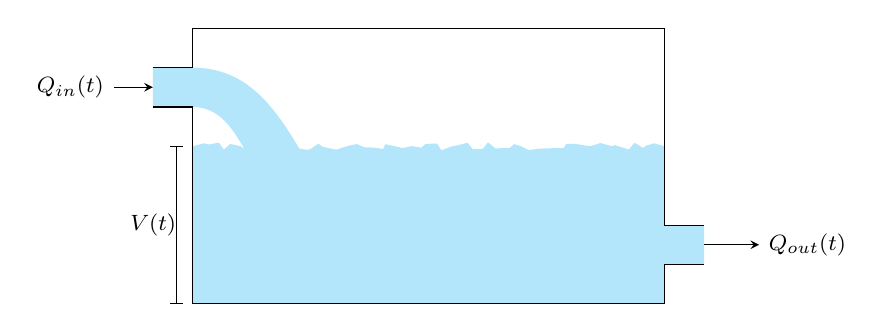
\begin{tikzpicture}
		\fill[cyan!30]
		decorate[ragged border]{
			(0,2) -- (6,2)
		}
		-- (6,1) -- (6.5,1) -- (6.5,0.5) -- (6,0.5) --(6,0) -- (0,0) -- cycle;
		\fill[cyan!30] (-0.5,2.5) -- (0,2.5) to[in=120,out=0](0.7,1.9)-- (1.4,1.9)
		to[out=120,in=0] (0,3) -- (-0.5,3) -- cycle;
		\draw (-0.5,2.5) -- (0,2.5) -- (0,0) -- (6,0) -- (6,0.5) -- (6.5,0.5);
		\draw (-0.5,3) -- (0,3) -- (0,3.5) -- (6,3.5) -- (6,1) -- (6.5,1);
		\draw[|-|] (-0.2,0) --
		node[fill=white,font=\footnotesize,inner ysep=2pt,inner
		xsep=0,anchor=east]{$V(t)$}(-0.2,2);
		\draw[stealth-] (-0.5,2.75) -- (-1,2.75)
		node[anchor=east,font=\footnotesize,align=right]{$Q_{in}(t)$};
		\draw[-stealth] (6.5,0.75) -- (7.2,0.75)
		node[anchor=west,font=\footnotesize]{$Q_{out}(t)$};
		\node[anchor=north,font=\footnotesize] at (3,3) {};
		\node[anchor=north,font=\footnotesize] at (3,2) {};
		\node[anchor=north,font=\footnotesize] at (3,1) {};
		\end{tikzpicture}
		\caption{The basic tank flow problem sees the a tank with a volume at some point in time, $V(t)$, with an inflow, $Q_{in}(t)$, and an outflow, $Q_{out}(t)$.}
	\end{minipage}
	\hspace{2cm}
	\begin{minipage}[t]{0.45\textwidth}
		\centering
		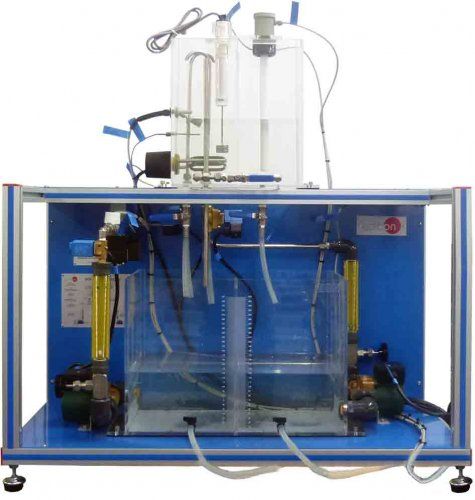
\includegraphics[scale=0.5]{lab_equip}
		\caption{Practical hardware consisted of an upper tank for the controlled fluid level, a lower water reservoir, a pump, and a controlled valve.}
	\end{minipage}
\end{figure}

The biggest problem arises when tuning the PID for a non-linear system. Parameters which work well for one operating point in the system are not guaranteed to work well for a different operating point. A classic example of this is seen when trying to control supersonic aircraft: the system behaves very differently in sub-sonic and super-sonic modes of flight. There three main parameters to consider when tuning a PID controller: the proportional gain ($K_c$), the integral gain ($T_i$), and the derivative gain ($T_d$). These parameters can be seen in the PID expression for the control action, $u(t)$, shown in equation (4).
\begin{equation}
	u(t) = K_c e(t) + T_i \int_{0}^{t}e(\tau) d \tau + T_d \frac{de(t)}{dt}
\end{equation}

Note that there are many different ways to express the PID controller mathematically - one of the most common is to use $\sfrac{K_c}{t_i}$ to represent $T_i$ and $K_c \cdot t_d$ to represent $T_d$. To maintain consistency with the software used in the practical, the equation shown in equation (4) is used. The PID controller is implemented using a feedback loop. This allows the control signal to be calculated using the difference between the set point and the measured output of process variable. A basic diagram of the topology can be seen in Figure 3.\\

\begin{figure}[h]
	\centering
	\begin{tikzpicture}[auto, node distance=2cm,>=latex']
	% We start by placing the blocks
	\node [input, name=input] {};
	\node [sum, right of=input] (sum) {};
	\node [block, right of=sum, node distance=2.5cm] (controller) {PID};
	\node [block, right of=controller, node distance=4cm] (system) {Plant};
	% We draw an edge between the controller and system block to 
	% calculate the coordinate u. We need it to place the measurement block. 
	\draw [->] (controller) -- node[name=u] {$u(t)$} (system);
	\node [output, right of=system, node distance=3cm] (output) {};
	\node [block, below of=u] (measurements) {Measurements};
	
	% Once the nodes are placed, connecting them is easy. 
	\draw [draw,->] (input) -- node {$V_{ref}$} (sum);
	\draw [->] (sum) -- node {$e(t)$} (controller);
	\draw [->] (system) -- node [name=y] {$V(t)$}(output);
	\draw [->] (y) |- (measurements);
	\draw [->] (measurements) -| node[pos=0.99] {$-$} node [near end] {$V_m(t)$} (sum);
	\end{tikzpicture}
	\caption{Classical engineering feedback control block diagram implemented for the modelled population system. Measurements in this hypothetical control system would come from government collected data on population which is prone to lag - this may require estimates to be used instead of true figures for the scheme to work.}
\end{figure}

The plant itself, shown in Figure 2, consisted of an upper tank with a water level sensor which was used as the tank for the fluid control practical. The lower tank simply served as a reservoir to catch the outflow. Water is pumped from the lower tank to the top tank using a pump. The flow rate can be controlled using either a manual valve or by a pneumatically actuated valve. Software was used to implement the control scheme. When activated the controller would actuate the pneumatic valve to change the inflow to the tank.

%----------------------------------------------------------------------------------------
%	Laboratory Control
%----------------------------------------------------------------------------------------

\section{Implementing P, PI, PD, and PID Control}

\subsection{Aim}
Study the system dynamics for tank flow under closed loop control. The control schemes that are tested in this section are proportional (P), proportional-integral (PI), proportional-derivative (PD), and proportional-integral-derivative (PID).

\subsection{Method}
The methods employed for testing each of the control schemes listed in the Aim are almost identical. Prior to the pump being turned on, the actuated valve is set approximately 30\% open. The small solenoid valve is opened to allow water to start flowing out of the tank, and simultaneously, the pump is activated which starts pumping water into the tank. The flow valve is adjusted to set the inflow rate to approximately 0.68$\si{\liter\per\minute}$, and the system is allowed to reach steady state. In most cases 120$\si{\milli\liter}$ was the system steady state. The step change was set to 10$\si{\milli\liter}$, and the control software was activated which captured time series data on tank fluid level and control actuation.

%----------------------------------------------------------------------------------------
%	Laboratory Proportional
%----------------------------------------------------------------------------------------
\subsection{Results}
This section outlines settings for each of the implemented controllers, along with a time series of the fluid level in the tank and the control actuation. Proportional control is in Subsection 3.3.1, Proportional-Integral control is in Subsection 3.3.2, Proportional-Derivative control is in Subsection 3.3.3, and full PID control is in Subsection 3.3.4. A full discussion of the performance of all of the controllers can be found in Section 3.4.

\newpage

\subsubsection{Proportional Control}

\begin{minipage}{0.45\textwidth}
Proportional control was implemented under two scenarios detailed in Table 1 to the right. In each test scenario the AVP valve was set to approximately 30\%. Time series data for the fluid level in the tank was captured for both scenarios, seen in Figures 4 and 6. The red time series shows the actuation profile over time for both scenarios - Figures 5 and 7 below. 
\end{minipage}
\hspace{1cm}
\begin{minipage}{0.45\textwidth}
	\captionof{table}{Control parameters and initial conditions for scenarios for proportional control}
	\small
	\begin{tabular}{lrr}
		\toprule
		 & Test 1 & Test 2 \\
		\midrule
		Starting Level & 145$\si{\milli\liter}$ & 100$\si{\milli\liter}$ \\
		Setpoint & 155$\si{\milli\liter}$ & 110$\si{\milli\liter}$ \\
		Flow Rate & 0.68$\si{\liter\per\minute}$ & 0.68$\si{\liter\per\minute}$ \\
		Proportional Gain ($K_c$) & 0.5 & 0.75 \\
		Integral Gain ($T_i$) & 0.0 & 0.0 \\
		Derivative Gain ($T_d$) & 0.0 & 0.0 \\
		\bottomrule
	\end{tabular}
\end{minipage}

\vspace{2cm}

\begin{figure}[h]
	\centering
	\begin{minipage}{0.45\textwidth}
		\centering
		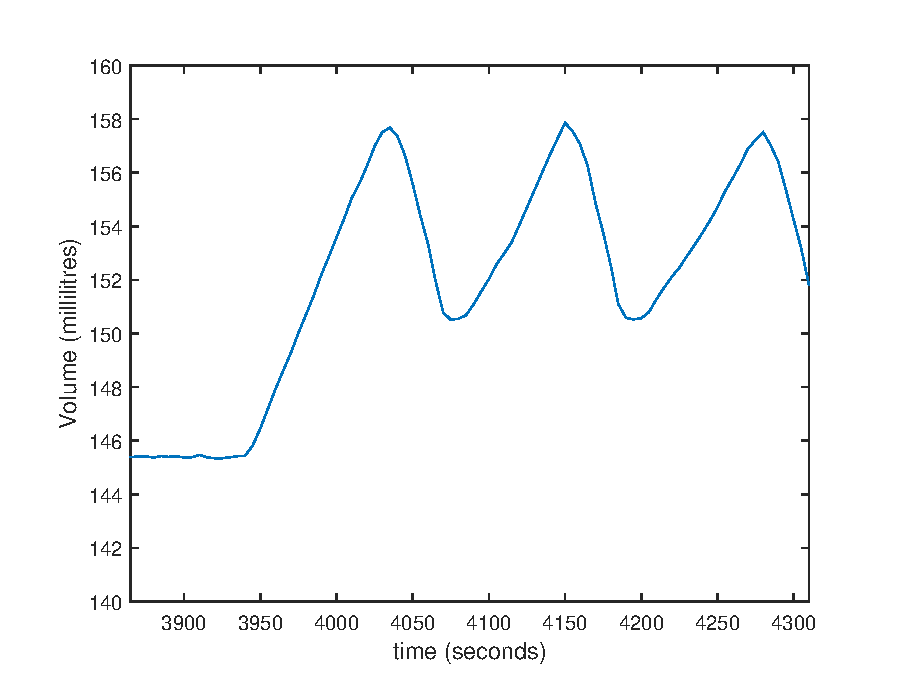
\includegraphics[scale=0.4]{P_Kc_05.eps}
		\caption{Time series plot of tank flow under proportional control with parameter $K_c$ set to 0.5}
	\end{minipage}
	\hspace{0.5cm}
	\begin{minipage}{0.45\textwidth}
		\centering
		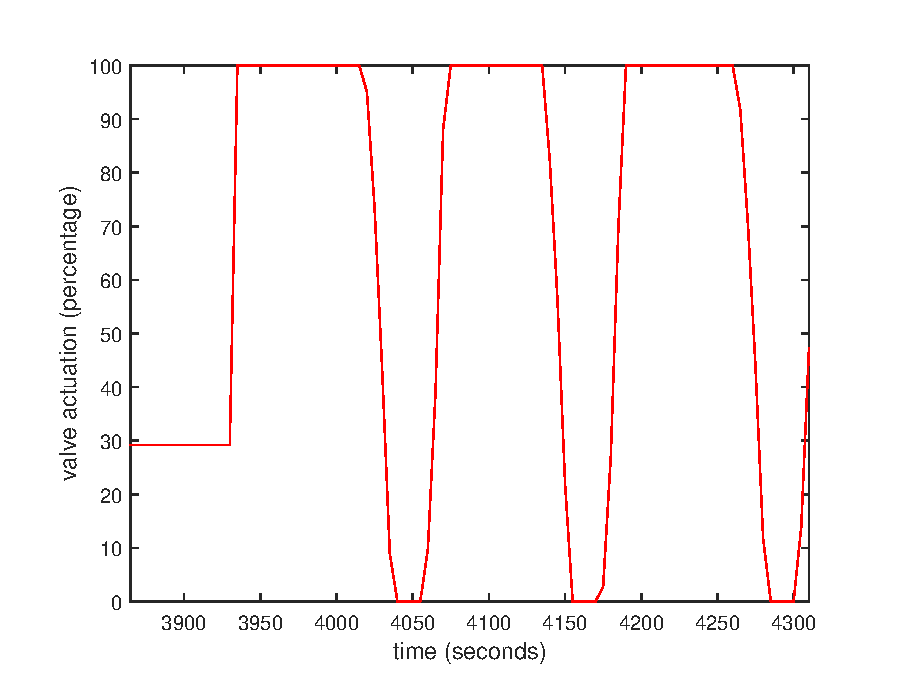
\includegraphics[scale=0.4]{P_Kc_05_control.eps}
		\caption{Time series plot of control actuation signal under proportional control with parameter $K_c$ set to 0.5}
	\end{minipage}
\end{figure}

\begin{figure}[h]
	\centering
	\begin{minipage}{0.45\textwidth}
		\centering
		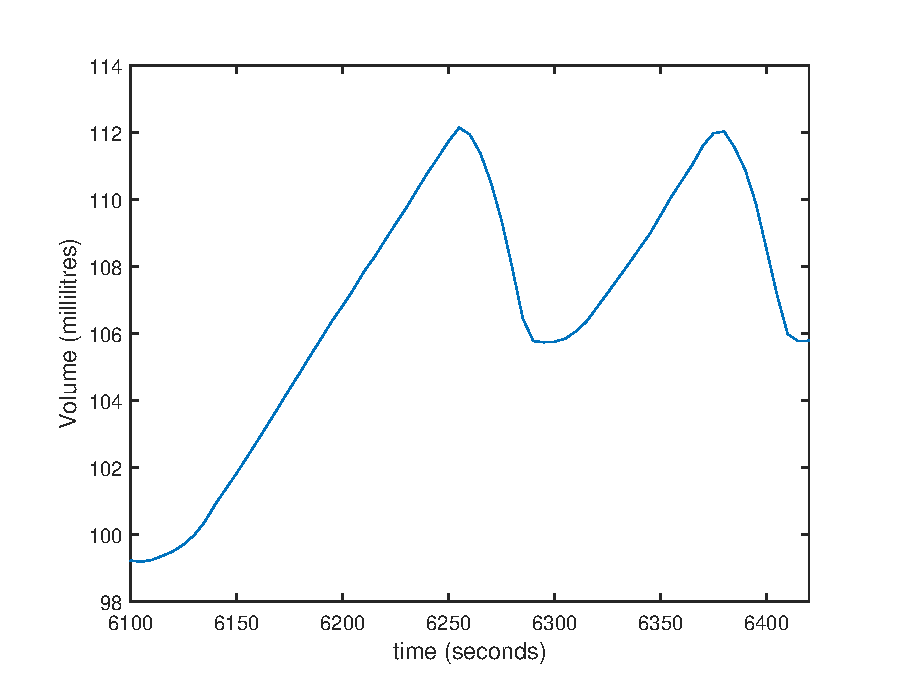
\includegraphics[scale=0.4]{P_Kc_075}
		\caption{Time series plot of tank flow under proportional control with parameter $K_c$ set to 0.75}
	\end{minipage}
	\hspace{0.5cm}
	\begin{minipage}{0.45\textwidth}
		\centering
		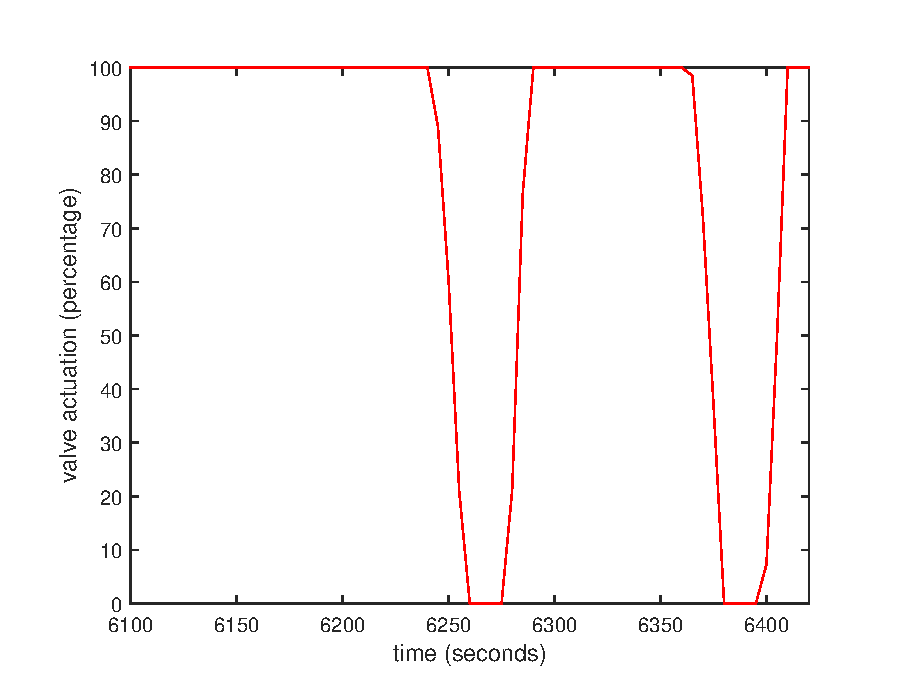
\includegraphics[scale=0.4]{P_Kc_075_control}
		\caption{Time series plot of control actuation signal under proportional control with parameter $K_c$ set to 0.5}
	\end{minipage}
\end{figure}

\clearpage

\subsubsection{Proportional Integral Control}

\begin{minipage}{0.4\textwidth}
	Proportional-integral control was implemented under three scenarios detailed in Table 2 to the right. In each test scenario the AVP valve was set to approximately 30\%. Time series data for the fluid level in the tank was captured for the scenarios, seen in Figures 8, 10, and 12. The red time series shows the actuation profile over time - Figures 9, 11, and 13 below. 
\end{minipage}
\hspace{0.5cm}
\begin{minipage}{0.45\textwidth}
	\captionof{table}{Control parameters and initial conditions for scenarios for proportional-integral control}
	\small
	\begin{tabular}{lrrr}
		\toprule
		& Test 1 & Test 2 & Test 3 \\
		\midrule
		Starting Level & 120$\si{\milli\liter}$ & 120$\si{\milli\liter}$ & 120$\si{\milli\liter}$ \\
		Setpoint & 130$\si{\milli\liter}$ & 130$\si{\milli\liter}$ & 130$\si{\milli\liter}$ \\
		Flow Rate & 0.65$\si{\liter\per\minute}$ & 0.64$\si{\liter\per\minute}$ & 0.66$\si{\liter\per\minute}$ \\
		Proportional Gain ($K_c$) & 0.5 & 0.5 & 0.5 \\
		Integral Gain ($T_i$) & 0.1 & 0.3 & 0.5 \\
		Derivative Gain ($T_d$) & 0.0 & 0.0 & 0.0 \\
		\bottomrule
	\end{tabular}
\end{minipage}

\begin{figure}[h]
	\centering
	\begin{minipage}{0.45\textwidth}
		\centering
		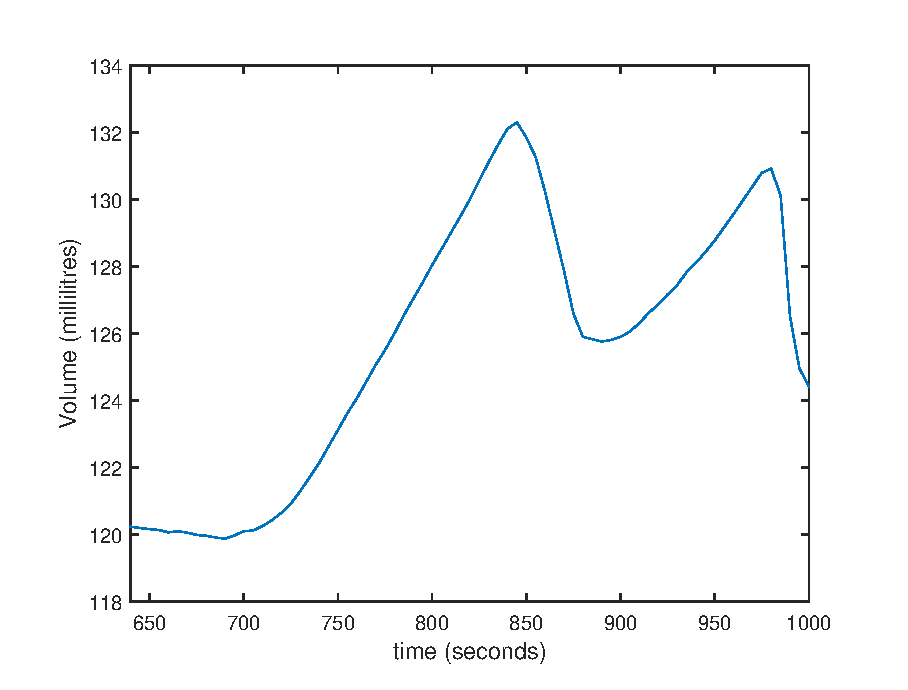
\includegraphics[scale=0.4]{PI_Kc_05_Ti_01}
		\caption{Time series tank flow under proportional control with $K_c = 0.5$, and $T_i = 0.1$}
	\end{minipage}
	\hspace{0.5cm}
	\begin{minipage}{0.45\textwidth}
		\centering
		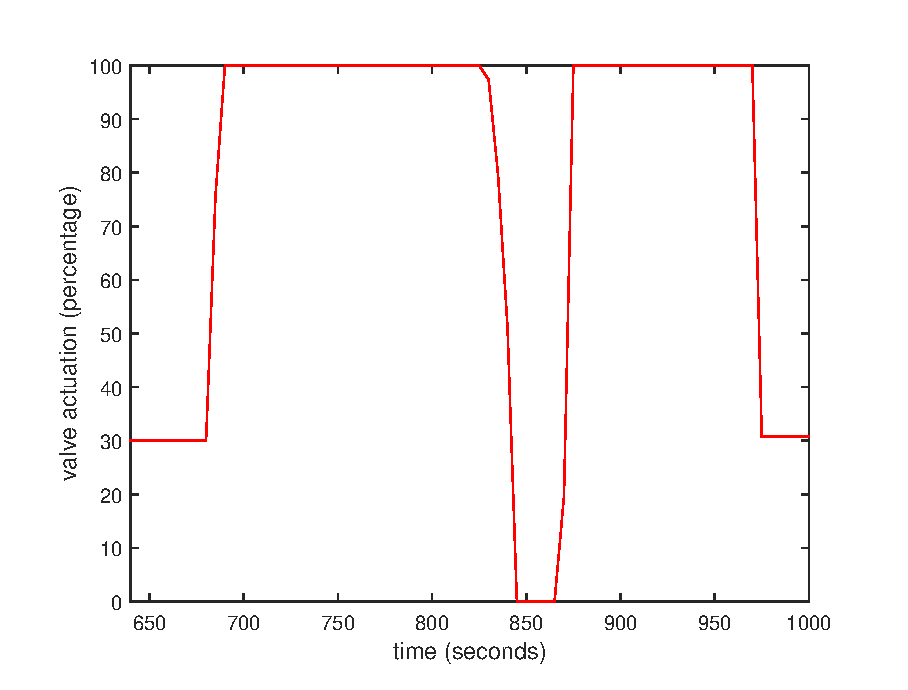
\includegraphics[scale=0.4]{PI_Kc_05_Ti_01_control}
		\caption{Time series proportional-integral control actuation with $K_c = 0.5$, and $T_i = 0.1$}
	\end{minipage}
\end{figure}

\begin{figure}[h]
	\centering
	\begin{minipage}{0.45\textwidth}
		\centering
		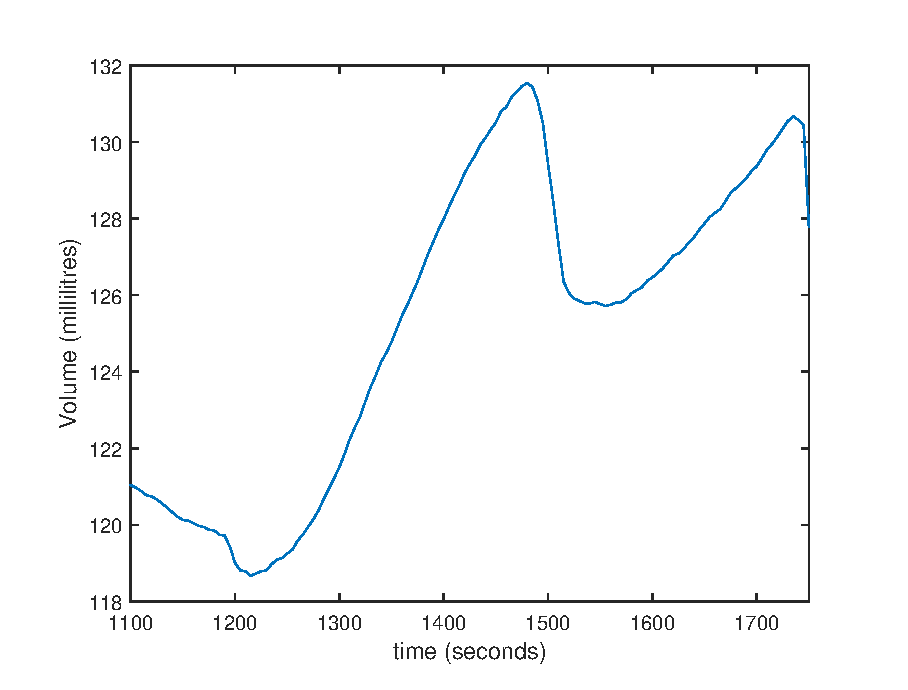
\includegraphics[scale=0.4]{PI_Kc_05_Ti_03}
		\caption{Time series tank flow under proportional control with $K_c = 0.5$, and $T_i = 0.3$}
	\end{minipage}
	\hspace{0.5cm}
	\begin{minipage}{0.45\textwidth}
		\centering
		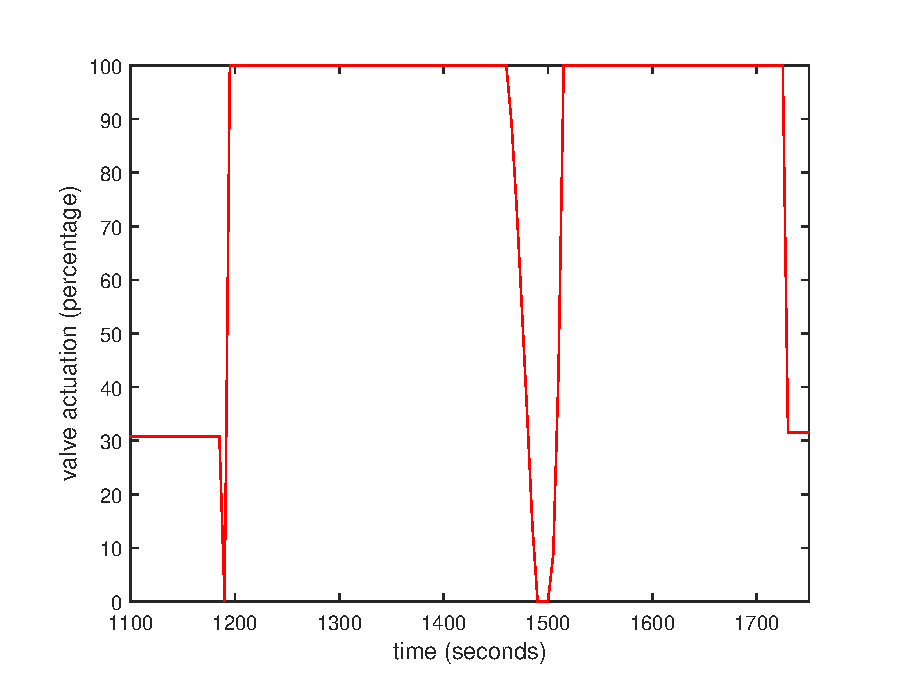
\includegraphics[scale=0.4]{PI_Kc_05_Ti_03_control}
		\caption{Time series proportional-integral control actuation with $K_c = 0.5$, and $T_i = 0.3$}
	\end{minipage}
\end{figure}

\begin{figure}[h]
	\centering
	\begin{minipage}{0.45\textwidth}
		\centering
		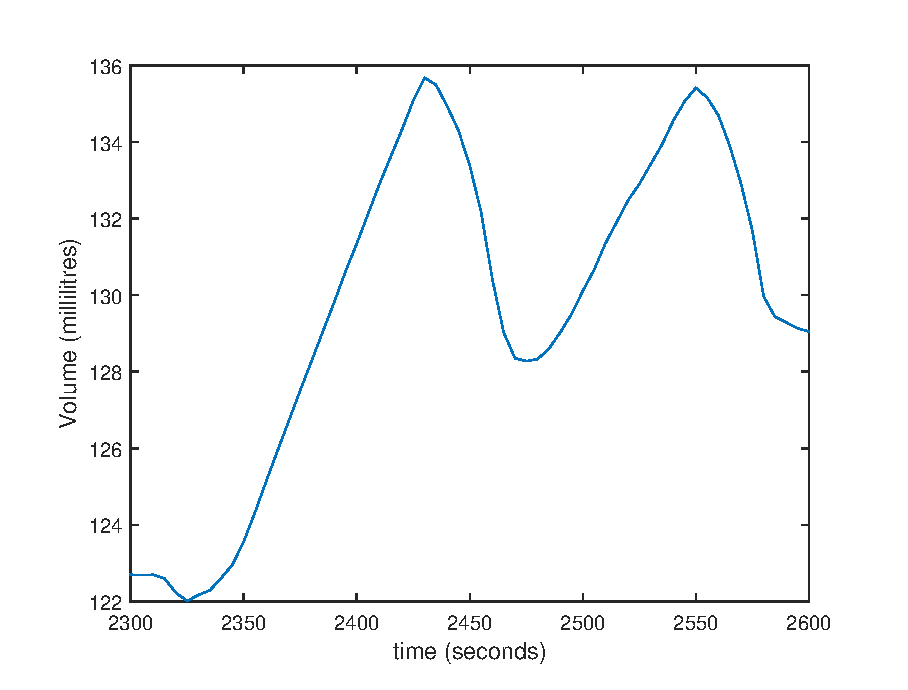
\includegraphics[scale=0.4]{PI_Kc_05_Ti_05}
		\caption{Time series tank flow under proportional control with $K_c = 0.5$, and $T_i = 0.5$}
	\end{minipage}
	\hspace{0.5cm}
	\begin{minipage}{0.45\textwidth}
		\centering
		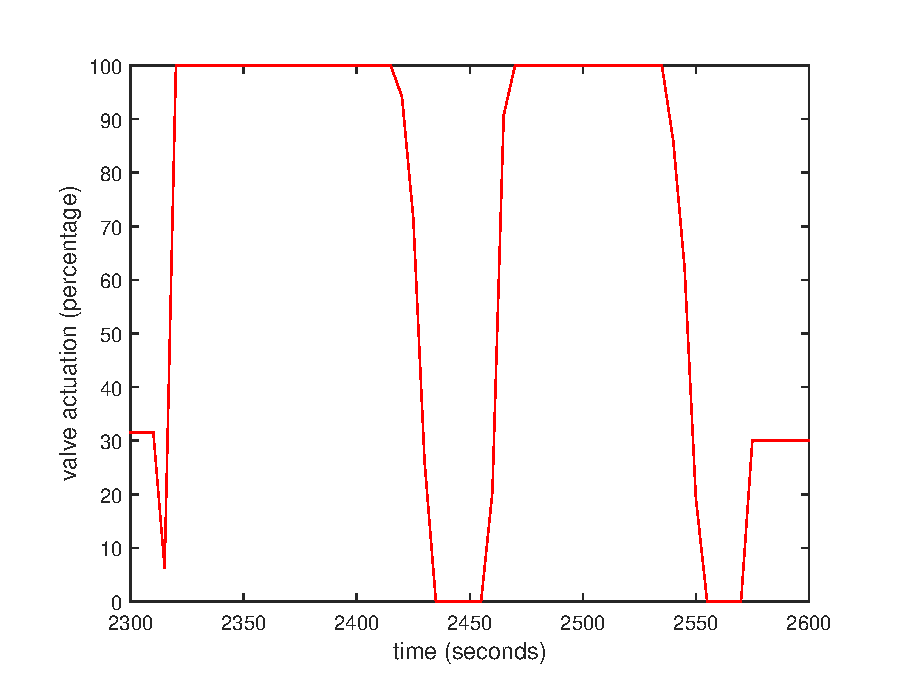
\includegraphics[scale=0.4]{PI_Kc_05_Ti_05_control}
		\caption{Time series proportional-integral control actuation with $K_c = 0.5$, and $T_i = 0.5$}
	\end{minipage}
\end{figure}

\clearpage

\subsubsection{Proportional Derivative Control}

\begin{minipage}{0.4\textwidth}
	Proportional-derivative control was implemented under three scenarios detailed in Table 3 to the right. In each test scenario the AVP valve was set to approximately 30\%. Time series data for the fluid level in the tank was captured for the scenarios, seen in Figures 14, 16, and 18. The red time series shows the actuation profile over time - Figures 15, 17, and 19 below. 
\end{minipage}
\hspace{0.5cm}
\begin{minipage}{0.45\textwidth}
	\captionof{table}{Control parameters and initial conditions for scenarios for proportional-derivative control}
	\small
	\begin{tabular}{lrrr}
		\toprule
		& Test 1 & Test 2 & Test 3 \\
		\midrule
		Starting Level & 120$\si{\milli\liter}$ & 120$\si{\milli\liter}$ & 120$\si{\milli\liter}$ \\
		Setpoint & 130$\si{\milli\liter}$ & 130$\si{\milli\liter}$ & 130$\si{\milli\liter}$ \\
		Flow Rate & 0.65$\si{\liter\per\minute}$ & 0.68$\si{\liter\per\minute}$ & 0.67$\si{\liter\per\minute}$ \\
		Proportional Gain ($K_c$) & 0.5 & 0.5 & 0.5 \\
		Integral Gain ($T_i$) & 0.0 & 0.0 & 0.0 \\
		Derivative Gain ($T_d$) & 0.1 & 0.3 & 0.7 \\
		\bottomrule
	\end{tabular}
\end{minipage}

\begin{figure}[h]
	\centering
	\begin{minipage}{0.45\textwidth}
		\centering
		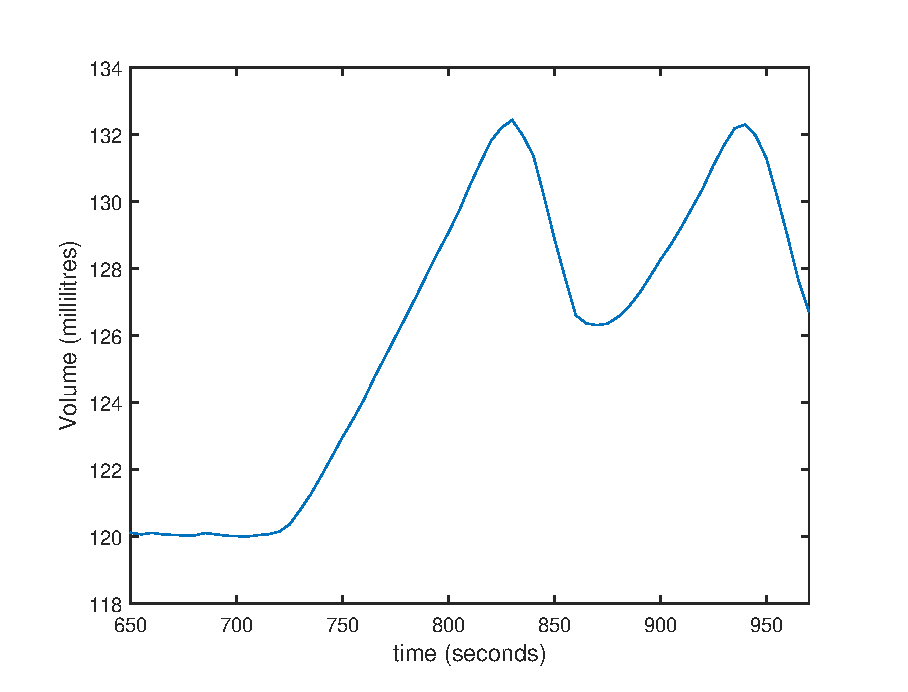
\includegraphics[scale=0.4]{PD_Kc_05_Td_03}
		\caption{Time series tank flow under proportional control with $K_c = 0.5$, and $T_d = 0.1$}
	\end{minipage}
	\hspace{0.5cm}
	\begin{minipage}{0.45\textwidth}
		\centering
		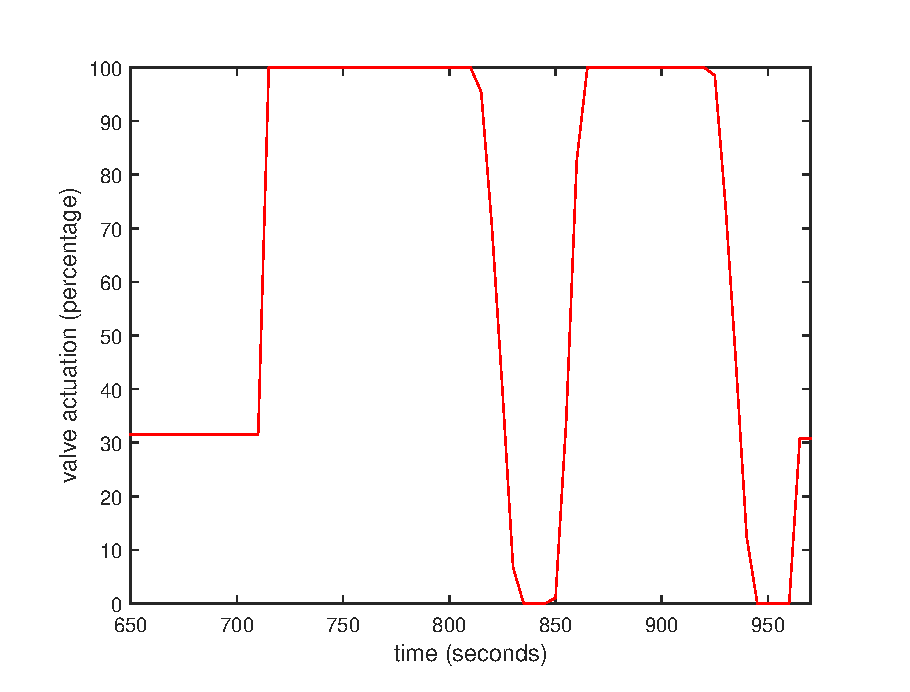
\includegraphics[scale=0.4]{PD_Kc_05_Td_03_control}
		\caption{Time series proportional-derivative control actuation with $K_c = 0.5$, and $T_d = 0.1$}
	\end{minipage}
\end{figure}

\begin{figure}[h]
	\centering
	\begin{minipage}{0.45\textwidth}
		\centering
		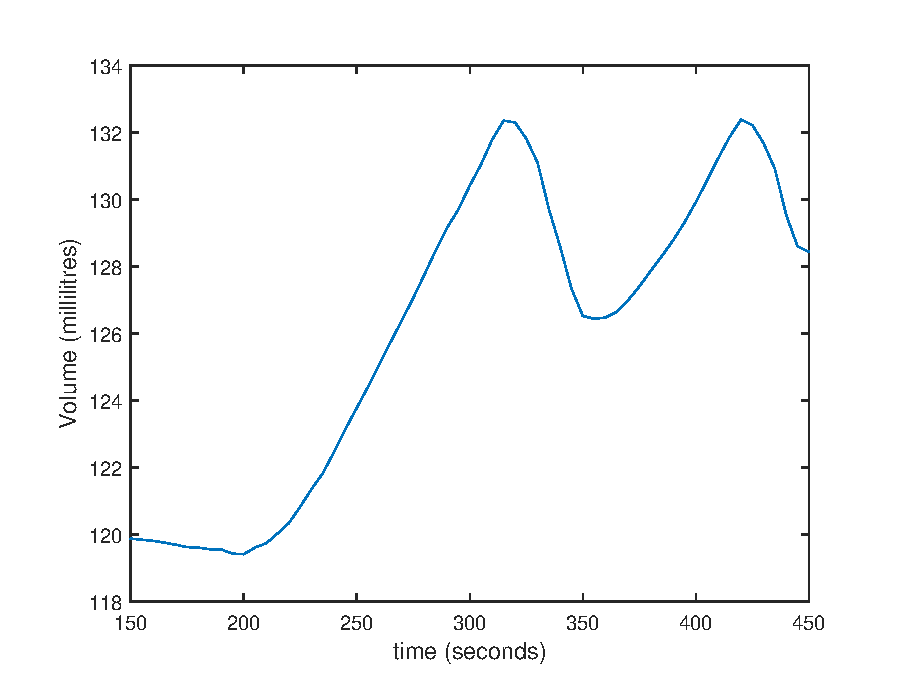
\includegraphics[scale=0.4]{PD_Kc_05_Td_05}
		\caption{Time series tank flow under proportional control with $K_c = 0.5$, and $T_d = 0.3$}
	\end{minipage}
	\hspace{0.5cm}
	\begin{minipage}{0.45\textwidth}
		\centering
		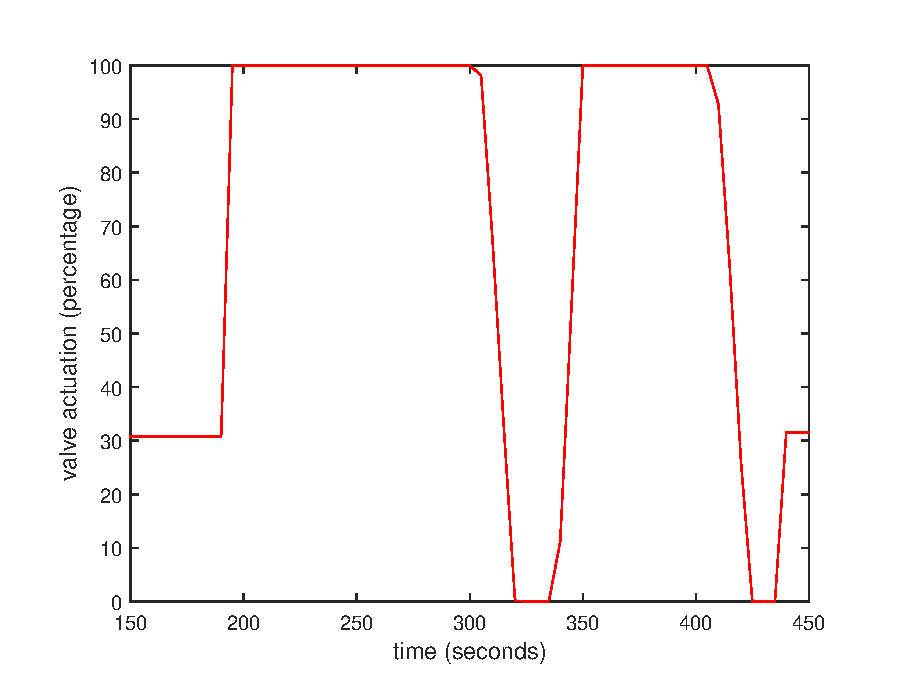
\includegraphics[scale=0.4]{PD_Kc_05_Td_05_control}
		\caption{Time series proportional-derivative control actuation with $K_c = 0.5$, and $T_d = 0.3$}
	\end{minipage}
\end{figure}

\begin{figure}[h]
	\centering
	\begin{minipage}{0.45\textwidth}
		\centering
		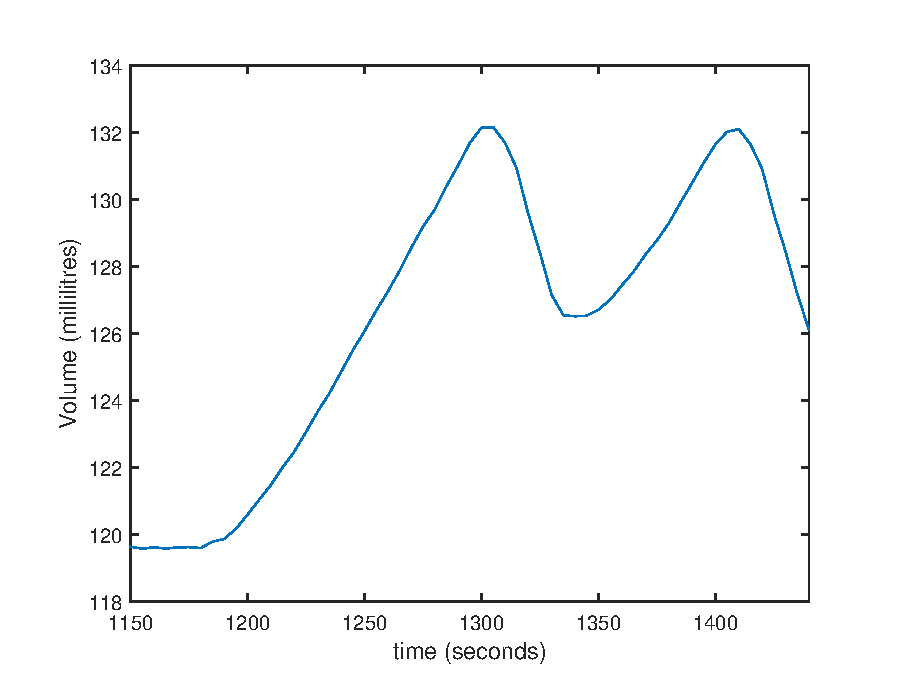
\includegraphics[scale=0.4]{PD_Kc_05_Td_07}
		\caption{Time series tank flow under proportional control with $K_c = 0.5$, and $T_d = 0.7$}
	\end{minipage}
	\hspace{0.5cm}
	\begin{minipage}{0.45\textwidth}
		\centering
		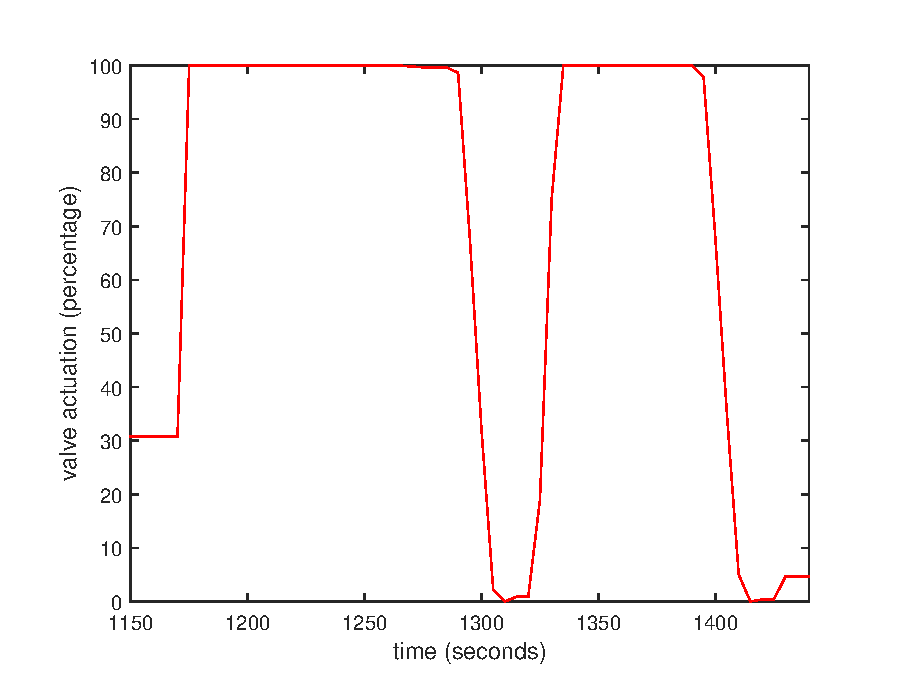
\includegraphics[scale=0.4]{PD_Kc_05_Td_07_control}
		\caption{Time series proportional-derivative control actuation with $K_c = 0.5$, and $T_d = 0.7$}
	\end{minipage}
\end{figure}

\clearpage

\subsubsection{Proportional, Integral, and Derivative Control}

\begin{minipage}{0.4\textwidth}
	PID control was implemented under three scenarios detailed in Table 4 to the right. In each test scenario the AVP valve was set to approximately 30\%. Time series data for the fluid level in the tank was captured for the scenarios, seen in Figures 20, 22, and 24. The red time series shows the actuation profile over time - Figures 21, 23, and 25 below.
\end{minipage}
\hspace{0.5cm}
\begin{minipage}{0.45\textwidth}
	\captionof{table}{Control parameters and initial conditions for scenarios for PID control}
	\small
	\begin{tabular}{lrrr}
		\toprule
		& Test 1 & Test 2 & Test 3 \\
		\midrule
		Starting Level & 121$\si{\milli\liter}$ & 120$\si{\milli\liter}$ & 120$\si{\milli\liter}$ \\
		Setpoint & 131$\si{\milli\liter}$ & 130$\si{\milli\liter}$ & 130$\si{\milli\liter}$ \\
		Flow Rate & 0.68$\si{\liter\per\min}$ & 0.68$\si{\liter\per\min}$ & 0.68$\si{\liter\per\min}$ \\
		Proportional Gain ($K_c$) & 0.5 & 0.8 & 1.2 \\
		Integral Gain ($T_i$) & 0.1 & 0.3 & 0.8 \\
		Derivative Gain ($T_d$) & 0.5 & 0.3 & 0.3 \\
		\bottomrule
	\end{tabular}
\end{minipage}

\begin{figure}[h]
	\centering
	\begin{minipage}{0.45\textwidth}
		\centering
		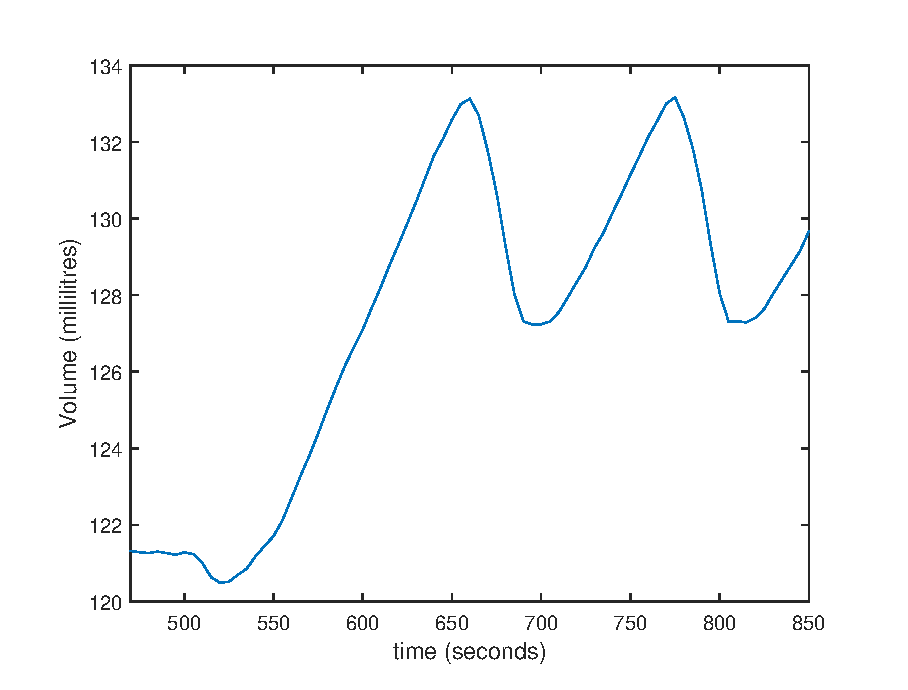
\includegraphics[scale=0.4]{PID_Kc_05_Ti_01_Td_05}
		\caption{Time series tank flow under PID control with $K_c = 0.5$, $T_i = 0.1$ and $T_d = 0.5$}
	\end{minipage}
	\hspace{0.5cm}
	\begin{minipage}{0.45\textwidth}
		\centering
		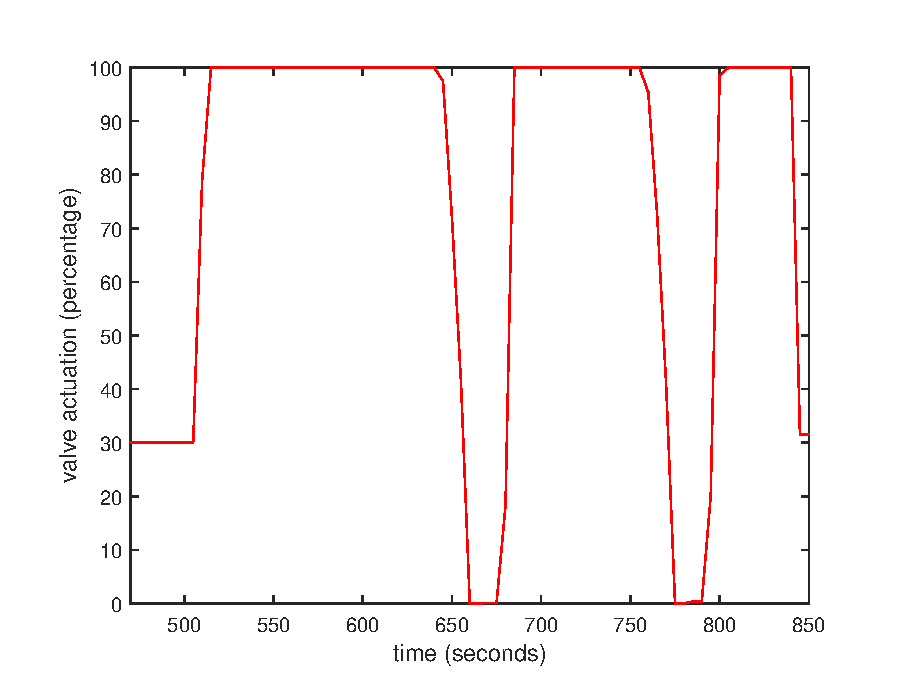
\includegraphics[scale=0.4]{PID_Kc_05_Ti_01_Td_05_control}
		\caption{Time series PID control actuation with $K_c = 0.5$, $T_i = 0.1$ and $T_d = 0.5$}
	\end{minipage}
\end{figure}

\begin{figure}[h]
	\centering
	\begin{minipage}{0.45\textwidth}
		\centering
		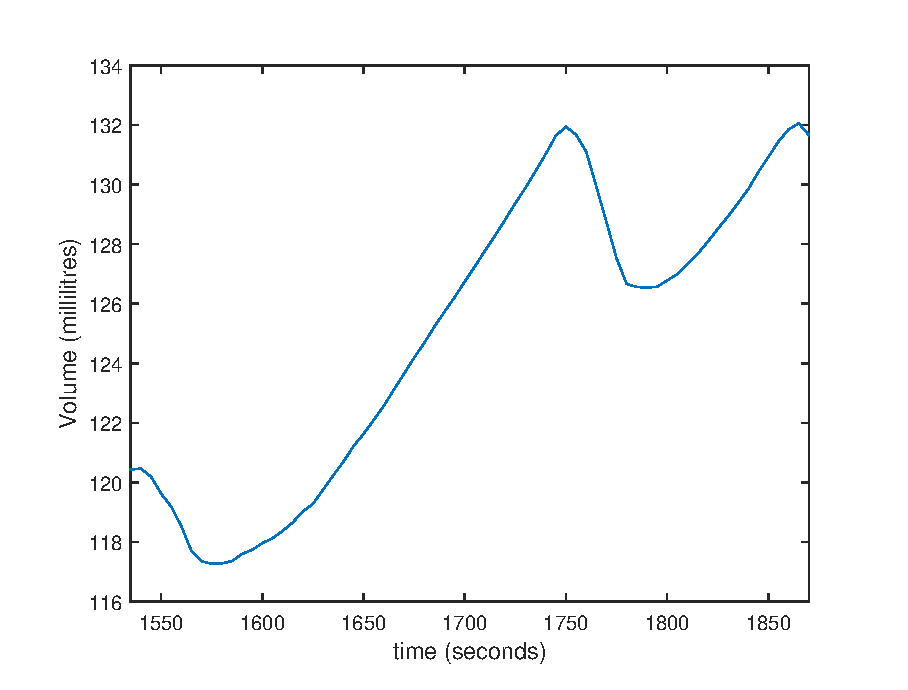
\includegraphics[scale=0.4]{PID_Kc_08_Ti_03_Td_03}
		\caption{Time series tank flow under PID control with $K_c = 0.8$, $T_i = 0.3$ and $T_d = 0.3$}
	\end{minipage}
	\hspace{0.5cm}
	\begin{minipage}{0.45\textwidth}
		\centering
		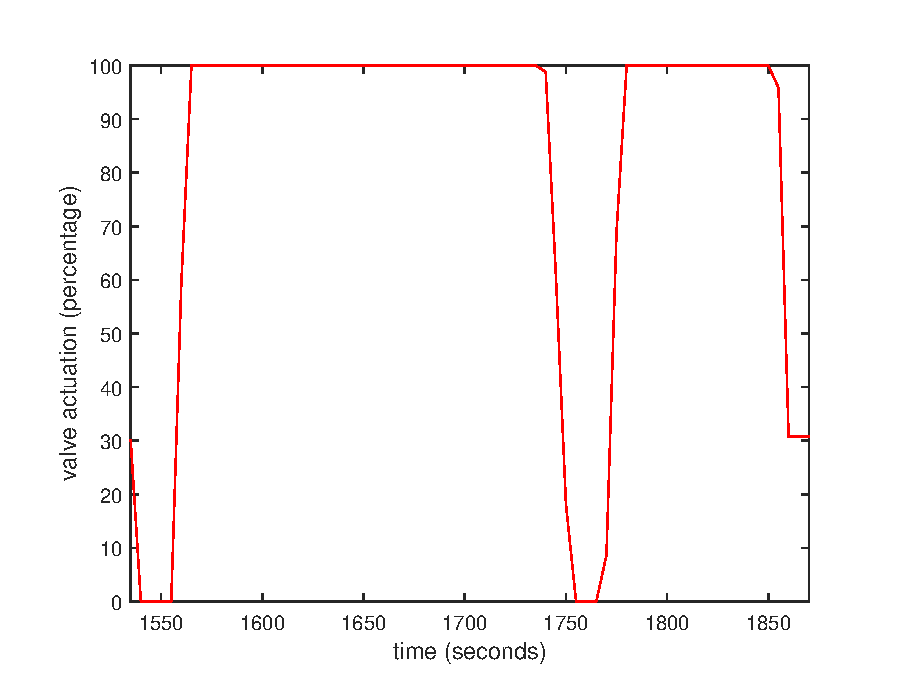
\includegraphics[scale=0.4]{PID_Kc_08_Ti_03_Td_03_control}
		\caption{Time series PID control actuation with $K_c = 0.8$, $T_i = 0.3$ and $T_d = 0.3$}
	\end{minipage}
\end{figure}

\begin{figure}[h]
	\centering
	\begin{minipage}{0.45\textwidth}
		\centering
		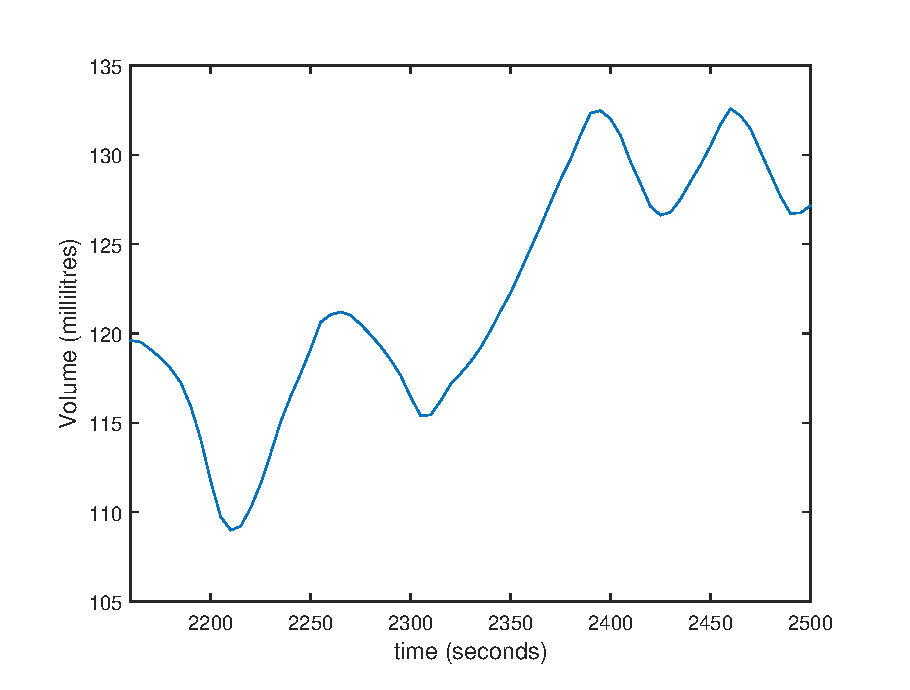
\includegraphics[scale=0.4]{PID_Kc_12_Ti_08_Td_03}
		\caption{Time series tank flow under PID control with $K_c = 1.2$, $T_i = 0.8$ and $T_d = 0.3$}
	\end{minipage}
	\hspace{0.5cm}
	\begin{minipage}{0.45\textwidth}
		\centering
		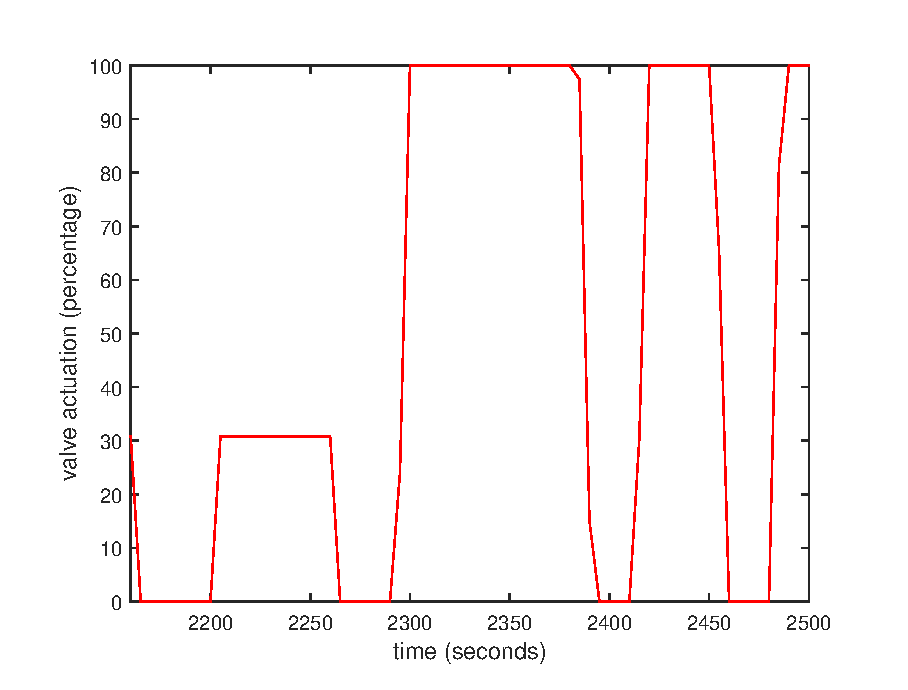
\includegraphics[scale=0.4]{PID_Kc_12_Ti_08_Td_03_control}
		\caption{Time series PID control actuation with $K_c = 1.2$, $T_i = 0.8$ and $T_d = 0.3$}
	\end{minipage}
\end{figure}

\subsection{Discussion}
Control was implemented with varying success. In each of the control types we see that the controller was able to maintain the fluid level of the tank within 2$\si{\milli\liter}$ of the desired value. The controller was able to reach the set point after about 50 seconds. Despite the apparent success, it must be noted that different outcomes were expected for different control schemes. This was not the case. Every control type including P, PI, PD, and PID saw similar control actuation profiles for the pneumatic valve. Subsequently, similar behaviour of the tank fluid level was observed for each control type. Further, within each of the different control schemes, we see almost identical control actuation and tank fluid levels for all variations of the parameters. The main exception here was when the proportional gain was set to 1.2 in Section 3.3.4 for the PID control - this resulted in some mild instability.\\

In every scenario, for every control scheme, we see a type of bang-bang control (also known as on-off control). This is a poor control outcome - it is energy inefficient and results in increased wear on the actuator. Interestingly, when the valve open 100\% the tank level increased, and when the valve was at 0\% the tank level decreased. This implies that, theoretically, there is a point somewhere between 0\% and 100\% in which the controller could maintain a steady state. We believe that the inability to reach this steady state is due to the pneumatic valve not being sensitive enough. Anecdotally, support for this claim can be found in  the observation that, on occasion, the valve would become stuck during actuation and cease moving until sufficient pressure had built up, at which point it would move very rapidly causing spikes in the actuation profile, like those seen in Figure 11 and Figure 13.

%----------------------------------------------------------------------------------------
%	Laboratory S-Curve Tuning
%----------------------------------------------------------------------------------------

\section{S-Curve Tuning}

\subsection{Aim}
Implement a PID controller using Ziegler-Nicols tuning to determine the parameters for the PID controller.

\subsection{Method}
The tank system is set to operate without any control in order to capture the open loop behaviour in response to a small step change. The small solenoid outflow valve was opened. The pump was engaged and the pneumatically controlled valve was set to 30\%. The manual valve on the flow meter was changed such that the flow was $0.68\si{\liter\per\minute}$, and the tank was allowed to reach its steady state of 120$\si{milli\liter}$. At 725 seconds a small positive step change of 5\% was introduced to the pneumatic valve, and the system response was recorded. A logistic curve was imposed over the captured open loop response data, adjusting the parameters for a visual fit. The logistic expression was used to calculated parameters $K_c$, $T_i$, and $T_d$ for the PID controller - calculations can be found in Section 4.3. Tuned PID performance was evaluated in a trial identical to that seen in Section 3.3.4.  

\subsection{Calculations}
\begin{minipage}{0.45\textwidth}
Captured open loop time response time series is shown Figure 26. The blue curve is the captured data. The plant system itself can be thought of as a first order system, and the instrument which measures the volume of water in the tank is also thought of as a first order system. Together they form a second order system, and as such we expect to see an S-curve, however, we simply see a first order $RC$ system response to the small step change on the open loop system. Despite the fact that the open loop dynamics are clearly not in the desired form, a logistic curve was forced onto the data. Note that typically when dealing with empirical evidence or data, a statistical method such as linear regression is taken to fit the model to the data, however, in this case given obvious mispecification of the logistic model to this data, the model was fit by hand, simply adjusting the parameters until the model fit visually.
\end{minipage}
\hspace{1cm}
\begin{minipage}{0.45\textwidth}
	\centering
	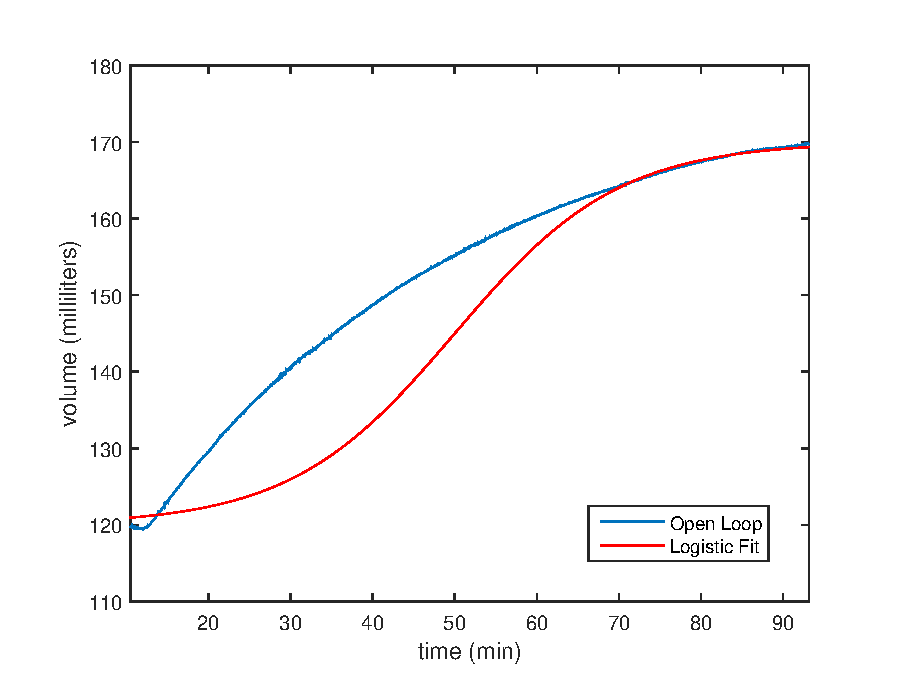
\includegraphics[scale=0.55]{scurve}
	\captionof{figure}{Open loop response to 5\% step change in pneumatic valve position, with imposed logistic curve to calculate PID parameters.}
\end{minipage}

\vspace{0.5cm}

The general form of a logistic model is given in equation (X) below. We note that $A$ is the lower asymptote, $K$ is the upper asymptote, $B$ is a parameter controlling how quickly the model transitions from the lower asymptote to the upper asymptote, and $h$ simply translates the model along the temporal axis.
\begin{equation}
	V(t) = A + \frac{K - A}{1 + e^{-B(t - h)}}
\end{equation}

Figure X clearly shows that the lower asymptote is 120 and the upper asymptote is 170. Parameters $B$ and $h$ were adjusted by hand to yield an approximate fit. The fit logistic equation is expressed mathematically in equation X, and shown graphically Figure X.
\begin{equation}
V(t) = 120 + \frac{50}{1 + e^{-0.1(t - 50)}} 
\end{equation}

To determine estimates for our PID controller parameters, we need to determine $R$ and $L$. The parameter $R$ is slope of the tangent to the fit logistic curve at the point where the horizontal line $V_{hz}(t) = 120 + 0.63A$ intersects the logistic curve. We note that $A$ is the difference between the upper and lower asymptotes. The parameter $L$ is the difference between step change transition time and the time at which the aforementioned tangent intersects the lower asymptote. These parameters are slightly esoteric in their definition, and part of this section is dedicated to their calculation to provide more transparency.

We first need to find the time, $t_A$, at which the horizontal line $V_{hz}(t) = 120 + 0.63A$ meets the fit logistic model, $V(t)$. This is given by solving:
\begin{align}
120 + 0.63 \times 50 &= 120 + \frac{50}{1 + e^{-0.1(t_A - 50)}}\\
151.50 &= 120 + \frac{50}{1 + e^{-0.1(t_A - 50)}}
\end{align} 

We note that $t_A = 55.32$. To find the slope of the logistic curve at this point, we need to take the derivative of $V(t)$. This is given by:
\begin{equation}
	\frac{dV(t)}{dt} = \frac{5 e^{-0.1(t-50)}}{(1 + e^{-0.1(t-50)})^2}
\end{equation}

Evaluating this at $t_A$ we get that:
\begin{equation}
	R = \frac{dV(t)}{dt}\Bigr|_{t=55.32} = 1.16
\end{equation}

Using the slope found in (9), and the tangent point to the logistic curve, $(55.32, 151.50)$, we can determine the equation of the tangent, shown in equation (X).
\begin{equation}
V_{tan}(t) = 1.16t + 87.32
\end{equation}

In order to find $L$, first we need to determine the point of intersection with the lower asymptote $V_{120}(t) = 120$. This is found as follows:
\begin{align}
V_{120}(t) &= V_{tan}(t)\\
120 &= 1.16t + 87.32
\end{align}

We note that the point of intersection between the tangent and the lower asymptote occurs at $t=1907.89$, and we calculate $L$ as follows:
\begin{equation}
	L = 28.17 - 12.08 = 16.08
\end{equation}

We note that the practical suggests that both $R$ and $L$ be expressed with minutes as the time units. Hence, after the conversion we get $R = 1.41$ and $L = 19.71$. Finally, these the PID parameters are calculated as follows:
\begin{equation}
P = \frac{83RL}{DP} = 309.63 \ \ \ \ \ \ I = \frac{L}{0.5} = 32.16 \ \ \ \ \ \ D = 0.5L = 8.04
\end{equation}


\subsection{Results}
\begin{minipage}{0.45\textwidth}
	PID control was implemented under two scenarios detailed in Table 5 to the right. In each test scenario the AVP valve was set to approximately 30\%. Time series data for the fluid level in the tank was captured for the scenarios, seen in Figures 27, and 29. The red time series shows the actuation profile over time - Figures 28, and 30 below. Note that the second test uses normalisations of the calculated parameters to ensure that the values are between 0 and 1.
\end{minipage}
\hspace{0.5cm}
\begin{minipage}{0.45\textwidth}
	\captionof{table}{Control parameters and initial conditions for scenarios for PID control}
	\small
	\begin{tabular}{lrr}
		\toprule
		& Test 1 & Test 2 \\
		\midrule
		Starting Level & 120$\si{\milli\liter}$ & 125$\si{\milli\liter}$ \\
		Setpoint & 130$\si{\milli\liter}$ & 135$\si{\milli\liter}$ \\
		Flow Rate & 0.68$\si{\liter\per\min}$ & 0.68$\si{\liter\per\min}$ \\
		Proportional Gain ($K_c$) & 309.63 & 0.88 \\
		Integral Gain ($T_i$) & 32.16 & 0.0919 \\
		Derivative Gain ($T_d$) & 8.04 & 0.022 \\
		\bottomrule
	\end{tabular}
\end{minipage}

\begin{figure}[h]
	\centering
	\begin{minipage}{0.45\textwidth}
		\centering
		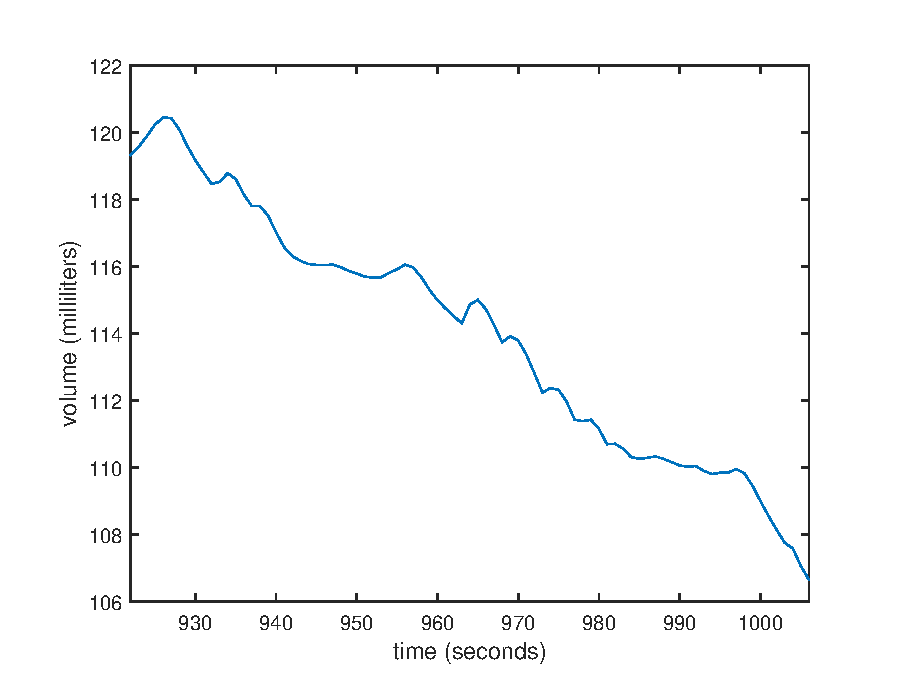
\includegraphics[scale=0.4]{s_curve_1_level}
		\caption{Time series tank flow under PID control with $K_c = 309.63$, $T_i = 32.16$ and $T_d = 8.04$}
	\end{minipage}
	\hspace{0.5cm}
	\begin{minipage}{0.45\textwidth}
		\centering
		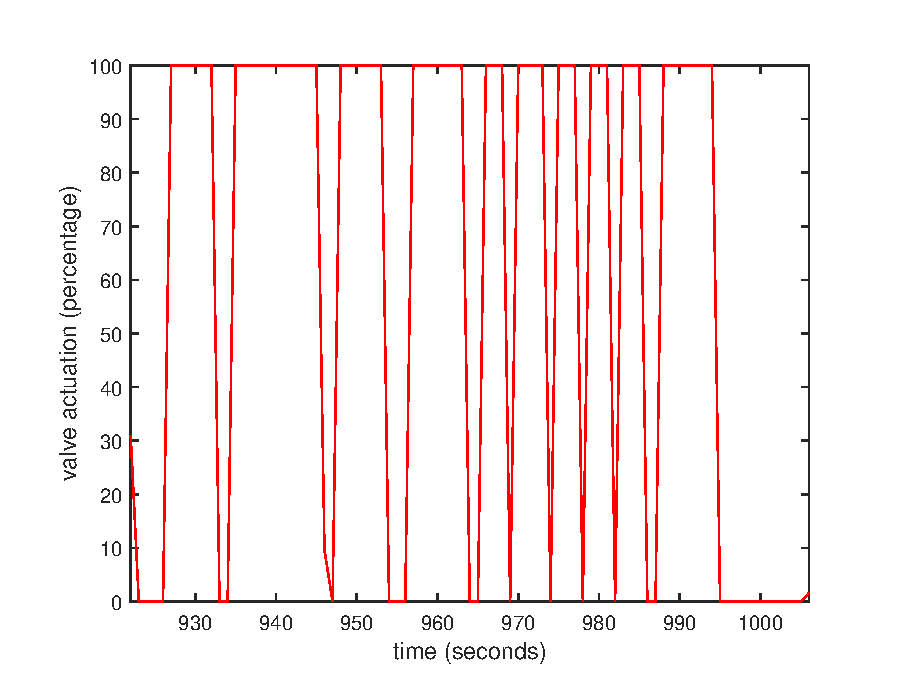
\includegraphics[scale=0.4]{s_curve_1_control}
		\caption{Time series PID control actuation with $K_c = 309.63$, $T_i = 32.16$ and $T_d = 8.04$}
	\end{minipage}
\end{figure}

\begin{figure}[h]
	\centering
	\begin{minipage}{0.45\textwidth}
		\centering
		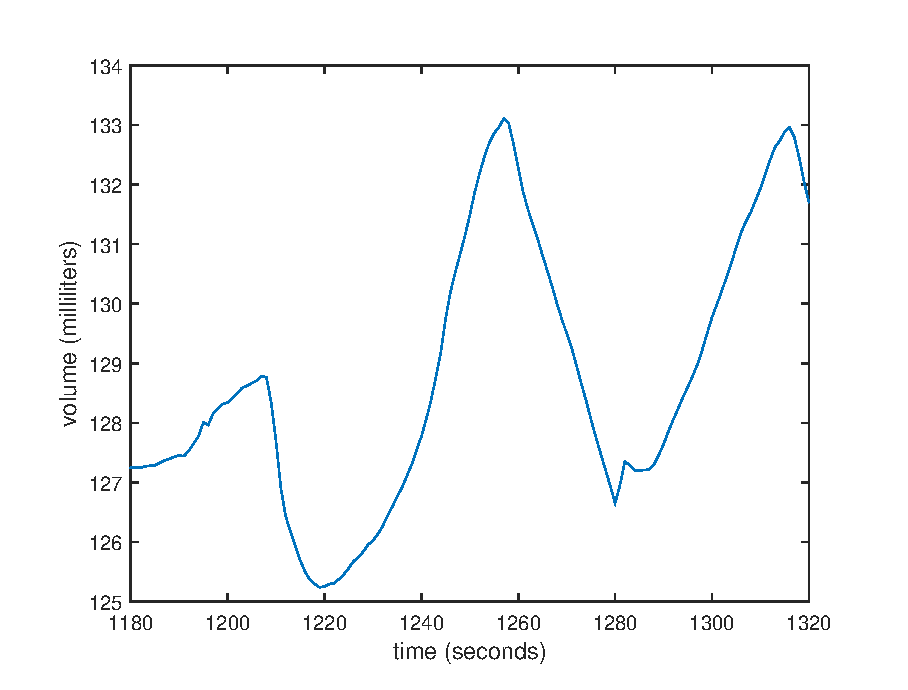
\includegraphics[scale=0.4]{s_curve_2_level}
		\caption{Time series tank flow under PID control with $K_c = 0.88$, $T_i = 0.0919$ and $T_d = 0.022$}
	\end{minipage}
	\hspace{0.5cm}
	\begin{minipage}{0.45\textwidth}
		\centering
		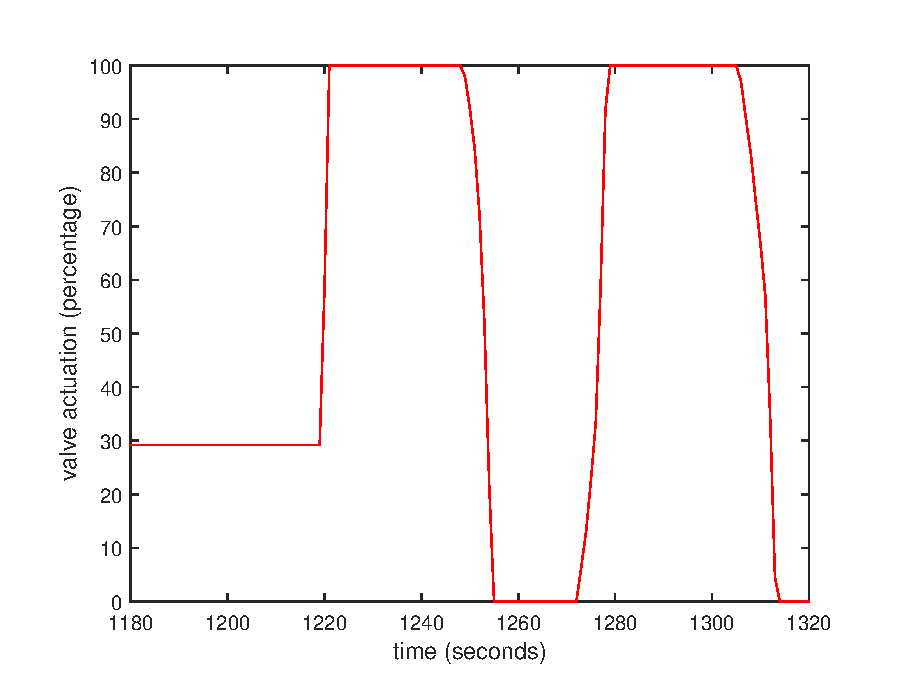
\includegraphics[scale=0.4]{s_curve_2_control}
		\caption{Time series PID control actuation with $K_c = 0.88$, $T_i = 0.0919$ and $T_d = 0.022$}
	\end{minipage}
\end{figure}

\subsection{Discussion}
The curve presented in Figure 26 from the open loop response to the step change is clearly not of the desired S-shape, which immediately calls into question the validity of the calculated parameters in this experiment. Supporting evidence of poor parameter estimation can be found in the sporadic control profile seen in Figure 28, and the inability of the controller under this scheme to properly control the fluid level in the tank. It was noted in Section 3.4 that parameter values above 1 seemed to introduce stability issues with the controller. In an attempt to mitigate this instability the calculated values were normalised, and the control test run again (as shown in Table 5 - Test 2). This adjustment to the parameters retains their values relative to each other. The controller, under the normalised regime, was able to control the tank fluid level at the desired set point, with approximately 2$\si{\milli\liter}$ fluctuations. Disappointingly, the control scheme with tuned parameters adopted the same bang-bang control profile as previous control schemes, and hence cannot be considered an improvement.

%----------------------------------------------------------------------------------------
%	Conclusion
%----------------------------------------------------------------------------------------

\section{Conclusion}
Each of the control schemes implemented for the tank system were able to provide some level of control. This is true for P, PI, PD, and PID. Notably, the controllers seemed to default to bang-bang control, irrespective of the values for the parameters. Interestingly, parameters given a value greater than 1 seemed to introduce instability into the controlled system. Finally, tuning PID parameters using Ziegler-Nicols S-curve method for systems which do not have the desired open-loop response curves provides poor control outcomes, in line with expectations.

\section{References}
\begin{itemize}
	\item Ogata, K. (2016). Modern control engineering. 5th ed. Pearson.
\end{itemize}



\end{document}